\documentclass[9pt, conference]{IEEEtran}
\IEEEoverridecommandlockouts

\usepackage{amsmath,amsfonts,graphicx}
\usepackage{amssymb,textcomp,mathtools}
\usepackage{bm,upgreek,algorithm,hyperref}
\usepackage{multirow,booktabs,hhline,array}
\usepackage{cite,url,makecell,setspace}
\usepackage{xcolor}
\pdfoutput=1

\def\thline{\noalign{\hrule height 1.0pt}}
\def\tthline{\noalign{\hrule height 1.4pt}}
\DeclareMathOperator*{\argmin}{argmin}
\DeclareMathOperator*{\argmax}{argmax}

\renewcommand{\vec}[1]{\bm{\mathrm{#1}}}
\def\x{{\mathbf x}}
\def\L{{\cal L}}

\title{Apollo: Band-sequence Modeling for High-Quality Audio Restoration}

\author{\IEEEauthorblockN{Kai~Li$^{\spadesuit,\clubsuit,*}$, Yi Luo$^{\clubsuit,*}$\\}
\IEEEauthorblockA{$^\spadesuit$Department of Computer Science and Technology, Tsinghua University, Beijing, China \\
$^\clubsuit$Tencent AI Lab, Shenzhen, China \\
tsinghua.kaili@gmail.com, oulyluo@tencent.com}
\thanks{$*$ The work was done while Yi Luo was at Tencent AI Lab and Kai Li was an intern there.}
}

\begin{document}
\maketitle

\begin{abstract}

\begin{abstract}
Language models (LMs), like other neural networks, often favor shortcut heuristics based on surface-level patterns.
Although LMs behave like n-gram models early in training, they must eventually learn hierarchical syntactic representations to correctly apply grammatical rules out-of-distribution (OOD).
In this work, we use case studies of English grammar to explore how complex, diverse training data drives models to generalize OOD. We construct a framework that unifies our understanding of random variation with training dynamics, rule selection with memorization, and data diversity with complexity. 
We show that these factors are nuanced, and that intermediate levels of diversity and complexity lead to inconsistent behavior across random seeds and to unstable training dynamics. 
Our findings emphasize the critical role of training data in shaping generalization patterns and illuminate how competing model strategies lead to inconsistent generalization outcomes across random seeds. Code is available at \url{https://github.com/sunnytqin/concept_comp.git}.

\end{abstract}

\end{abstract}
\begin{IEEEkeywords}
Audio restoration, audio superresolution, bandwidth extension, generative adversarial network 
\end{IEEEkeywords}
\section{Introduction}
\label{sec:introduction}
\section{Introduction}
\label{sec:introduction}

\begin{wrapfigure}{r}{0.5\textwidth}
\vspace{-6mm}
\begin{center}
    \includegraphics[width=0.5\textwidth]{images/cover.pdf}
  \end{center}
  \vspace{-4mm}
  \caption{\textbf{Overview of \implname.} In training, we tune the singular values of the weight matrices to generate a set of ``expert'' vectors specializing in different tasks. In inference, a two-pass process is adopted where the first applies the expert and the second generates the answer.}
  \label{fig:cover}
  \vspace{-4mm}
\end{wrapfigure}

Self-adaptive large language models (LLMs) would represent a significant advancement in artificial intelligence, enabling real-time adaptation to various tasks and contexts.
While compositionality and scalability are crucial for effective adaptation, current LLM training methodologies fall short of achieving both these properties simultaneously.
Our research aims to present a solution to address these gaps.

In principle, the first step toward achieving self-adaptive LLMs can be realized through the development of specialized expert modules, each fine-tuned~\citep{kaplan2020scaling} via techniques such as low-rank adaptation (LoRA)~\citep{hu2021lora}. 
However, several challenges need to be addressed to make this approach both scalable and compositional: (1) multiple expert modules significantly increase the number of parameters; (2) expert modules are often prone to overfitting; and (3) flexible composition of these experts is still an open problem.

To overcome these limitations, we first propose \svdacro, a novel parameter-efficient fine-tuning (PEFT) method to obtain effective building blocks for self-adaptation.
\svdacro works by extracting and selectively tuning only the singular values within the model's weight matrices.
By focusing on this essential and principled parameterization, our approach mitigates the risk of overfitting, drastically reduces computational demands, and allows for inherent compositionality.

We then introduce our full \implname framework, which entails a two-pass inference mechanism to produce dynamically adapted weights targeted for the test-time conditions (Figure~\ref{fig:cover}).
We design three different adaptation strategies that can be used within \implname, which we show provide monotonic performance benefits with increasing access to the test-time conditions.
We evaluate \svdacro and the full \implname framework through extensive experiments across a diverse range of LLMs and tasks.
\svdacro outperforms traditional efficient fine-tuning methods like LoRA on domain-specific datasets with far fewer parameters. 
\implname further improves performance, even for out-of-distribution tasks like visual QA. 
Our analysis even shows that \implname allows the reuse of \svdacro experts across different LLMs. In summary, our key technical contributions are: 
\vspace{-2mm}
\begin{itemize}
\item The development of \implname as a pivotal self-adaptation framework for LLMs, providing a blueprint to adapt the behavior of LLMs from a growing set of pre-trained skills.
\item The introduction of \svdacro, a novel PEFT method trainable with RL on small datasets, producing compact expert vectors with inherent compositionality.
\item The implementation of three adaptation strategies, effectively dispatching \svdacro-trained experts with properties designed to cope with different deployment scenarios.
\end{itemize}

\vspace{-2mm}

\section{Apollo}
\label{sec:model}
\subsection{Overall Pipeline}
\label{sec:overall}
Fig.\ref{fig:refiner}(a) presents the proposed Apollo pipeline. Apollo operates in the time-frequency domain and comprises a band-split module, a band-sequence modeling module, and a band-reconstruction module. Specifically, given compressed or distorted audio $\mathbf{S}\in \mathbb{R}^{1\times L}$, we first transfer $\mathbf{S}$ to its time-frequency domain representation $\mathbf{X}\in \mathbb{C}^{F\times T}$ using the Short-Time Fourier Transform (STFT), where $L$ denotes the length of audio, $F$ and $T$ denote the number of frequency bins and frames, respectively. Then, the band-split module maps to sub-band embeddings $\mathbf{Z}\in \mathbb{R}^{N\times T}$ using gain-shape representations $\mathbf{G}\in \mathbb{R}^{3\times M\times T}$ for each sub-band, where $N$ and $M$ denote the number of channels in sub-band embeddings and gain-shape representations, respectively. Next, the band-sequence modeling module performs joint modeling of temporal and sub-band using a stacked architecture based on Roformer \cite{su2024roformer} and temporal convolutional network (TCN) \cite{bai2018empirical,li2022efficient}. Finally, the band-reconstruction module converts the output $\mathbf{Q}\in \mathbb{R}^{N\times T}$ of the band-sequence modeling module into the reconstructed complex-valued spectrogram $\mathbf{Y}\in \mathbb{C}^{F\times T}$. It uses the inverse Short-Time Fourier Transform (iSTFT) to convert $\mathbf{Y}$ to a waveform $\bar{\mathbf{S}}\in \mathbb{R}^{1\times L}$.

\begin{table*}[]
\footnotesize
\centering
\caption{The structure of the STFT discriminator network.}
\begin{tabular}{cccccccc}
\toprule
\textbf{Layer Index} & \textbf{Layer Type}   & \textbf{Input Channels} & \textbf{Output Channels} & \textbf{Kernel Size} & \textbf{Padding} & \textbf{Stride} & \textbf{Activation} \\ \midrule
1                    & SpectralNorm + Conv2d & $F$                       & $F$                        & (3, 3)               & (1, 1)           & (1, 1)          & LeakyReLU(0.2)      \\
2                    & SpectralNorm + Conv2d & $F$                       & $F\times 2$              & (3, 3)               & (1, 1)           & (2, 2)          & LeakyReLU(0.2)      \\
3                    & SpectralNorm + Conv2d & $F\times 2$             & $F\times 4$              & (3, 3)               & (1, 1)           & (1, 1)          & LeakyReLU(0.2)      \\
4                    & SpectralNorm + Conv2d & $F\times 4$             & $F\times 8$              & (3, 3)               & (1, 1)           & (2, 2)          & LeakyReLU(0.2)      \\
5                    & SpectralNorm + Conv2d & $F\times 8$             & $F\times 16$             & (3, 3)               & (1, 1)           & (1, 1)          & LeakyReLU(0.2)      \\
6                    & SpectralNorm + Conv2d & $F\times 16$            & $F\times 32$             & (3, 3)               & (1, 1)           & (2, 2)          & LeakyReLU(0.2)      \\
7                    & Conv2d                & $F\times 32$            & 1                        & (3, 3)               & (1, 1)           & (1, 1)          & None               \\ \bottomrule
\end{tabular}
\label{tab:dis}
\vspace{-10pt}
\end{table*}

\subsection{Band-split Module}
As shown in Fig.\ref{fig:refiner}(b), given compressed or distorted audio spectrogram $\mathbf{X}$, we first split its frequency dimension $F$ into $K$ sub-band spectrograms $\{\mathbf{X}_k\in \mathbb{C}^{M_k\times T} | k\in [1, K]\}$. Inspired by the Gull codec \cite{luo2024gull}, we extract gain-shape representations $\mathbf{G}_k\in \mathbb{R}^{3\times M_k\times T}$ for each sub-band spectrogram:
\begin{equation}
\begin{aligned}
\mathbf{G}_{k} = \operatorname{Concat} \left[ 
\frac{\operatorname{Re}(\mathbf{X}_{k})}{\|\mathbf{X}_{k}\|_2}, \ 
\frac{\operatorname{Im}(\mathbf{X}_{k})}{\|\mathbf{X}_{k}\|_2}, \ 
\log\left(\|\mathbf{X}_{k}\|_2\right),
\right]
\end{aligned}
\end{equation}
where $\operatorname{Re}(\mathbf{X}_{k})$ and $\operatorname{Im}(\mathbf{X}_{k})$ denote the real and imaginary parts, respectively. $\|\mathbf{X}_{k}\|_2$ represents the $\ell_2$-norm of $\mathbf{X}_{k}$, given by:
\begin{equation}
    \|\mathbf{X}_{k}\|_2 = \sqrt{\operatorname{Re}(\mathbf{X}_{k})^2 + \operatorname{Im}(\mathbf{X}_{k})^2}
\end{equation}
$\log\left(\|\mathbf{X}_{k}\|_2\right)$ is the logarithm of the $\ell_2$-norm of $\mathbf{X}_{k}$. $\operatorname{Concat}$ refers to the concatenation of components. The gain-shape representation decouples the sub-band spectrogram's content and energy, allowing the reconstruction model to learn appropriate mappings that preserve the audio content. Subsequently, we map the gain-shape representations $\mathbf{G}$ into high-dimensional embeddings $\mathbf{Z}$ through a bottleneck layer, which consists of RMSNorm \cite{zhang2019root} and a 1D convolutional layer.

\subsection{Band-sequence Modeling Module}
In Apollo, we employ stacked Band-sequence modeling modules (BS modules, Fig.\ref{fig:refiner}(c)) to perform joint sub-band and temporal modeling with a stacking depth of $B$. Unlike BSRNN \cite{luo2023music} and Gull \cite{luo2024gull}, each BS module consists of a series of residual Roformers \cite{su2024roformer} and TCNs, which sequentially scan along the sub-band and time dimensions, and can increase the modeling capacity to improve the model performance. First, the residual Roformer is applied to the input $\mathbf{Z}$ along the frequency band dimension $K$ to obtain $\mathbf{Z}'\in \mathbb{R}^{N\times T}$, capturing global dependencies between sub-bands while preserving the local characteristics of the frequency domain signals. Next, the TCN is applied along the time dimension $T$ on $\mathbf{Z}'$ to generate the output $\mathbf{Q}\in \mathbb{R}^{N\times T}$. Since the $K$ sub-band features share the same feature dimension $N$, they all share a single TCN. The TCN consists of three convolutional blocks, each containing three convolutional layers. This design allows the TCN module to efficiently handle short-term dependencies and local temporal dynamics in audio signals, enhancing the model's ability to capture and understand temporal domain features.

\subsection{Band-reconstruction Module}
The output $\mathbf{Q}$ is passed through sub-band-specific fully connected (FC) layers to generate the estimated real and imaginary parts of the restored sub-band spectrograms (see Fig.\ref{fig:refiner}(d)). We utilize RMSNorm as the normalization layer within the fully connected layers and employ Gated Linear Units (GLUs) as the nonlinear activation function. Subsequently, the $K$ reconstructed sub-band spectrograms are concatenated along the frequency dimension to form the final reconstructed complex-valued spectrogram $\mathbf{Y}$. Finally, the reconstructed complex-valued spectrogram $\mathbf{Y}$ is converted back to the waveform domain $\bar{\mathbf{S}}$ through the iSTFT.

\begin{figure*}[h]
	\small
	\centering
	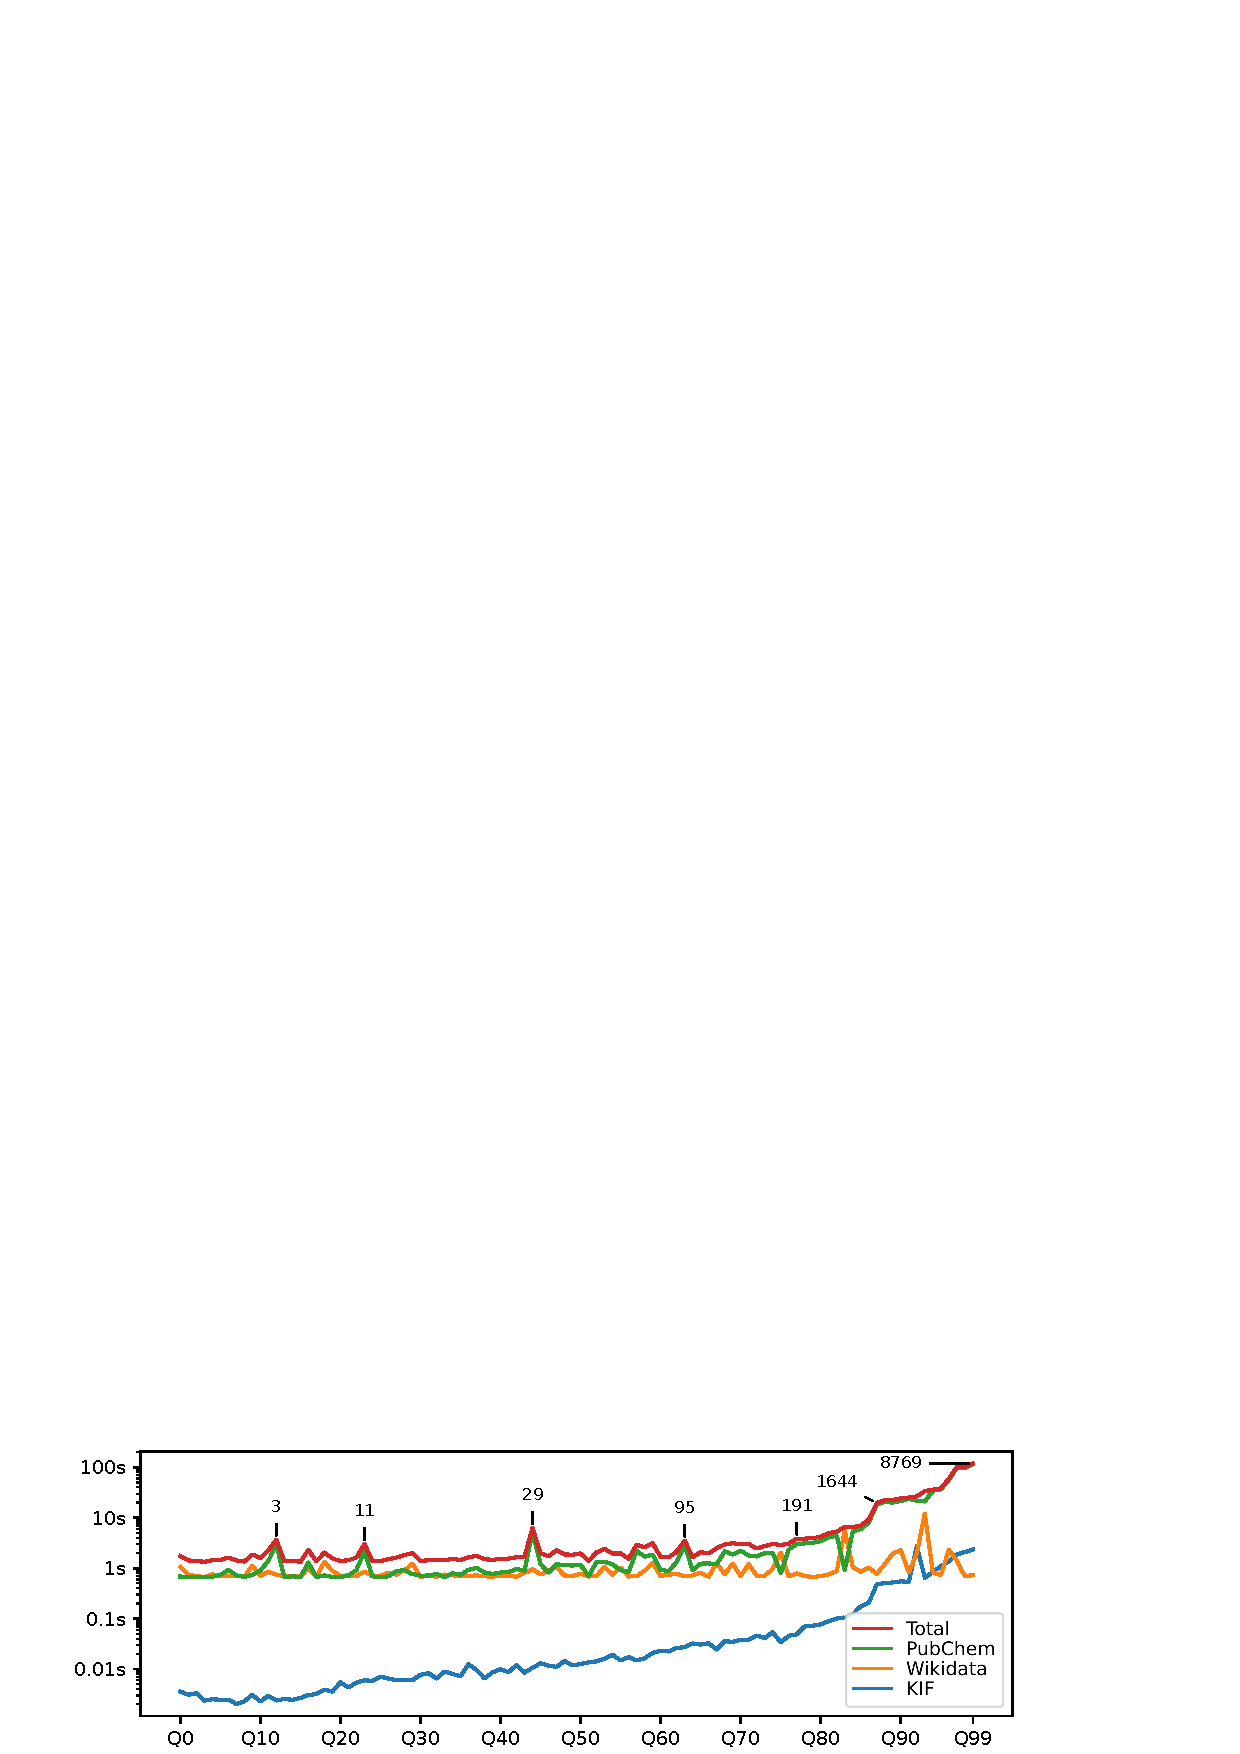
\includegraphics[width=2.0\columnwidth]{Figures/plot.pdf}
	\caption{Apollo and SR-GAN's SDR, SI-SNR and ViSQOL result in comparison at different bitrates.}
	\label{fig:plot}
\end{figure*}

\begin{table*}[]
\footnotesize
\centering
\caption{Different methods' SDR/SI-SNR/VISQOL scores for various types of music, as well as the number of model parameters and GPU inference time. For the GPU inference time test, a music signal with a sampling rate of 44.1 kHz and a length of 1 second was used.}
\begin{tabular}{cccccccc}
\toprule
Model  & Vocal            & Single Stem      & Multi-Stems      & Multi-Stems+Vocal & Overall   & Params (M) & RTF (ms)      \\ \midrule
SR-GAN \cite{lattner2021stochastic} & 10.62/9.19/2.72  & 13.88/12.52/3.28 & 14.92/14.16/3.41 & 16.87/15.54/3.76  & 14.07/12.85/3.29 & 322.53 & \textbf{34.55}\\
Apollo (Ours) & \textbf{13.99/12.58/3.44} & \textbf{16.56/15.99/4.08} & \textbf{17.52/17.15/4.41} & \textbf{18.51/18.26/4.54}  & \textbf{16.64/16.00/4.12} & \textbf{16.54} & 53.23 \\ \bottomrule
\end{tabular}
\label{tab:stems}
\vspace{-10pt}
\end{table*}

\subsection{Training Objection}
The proposed Apollo model is trained using a GAN framework to enhance the quality of audio restoration. Specifically, the discriminator network is inspired by the multi-resolution STFT discriminator, similar to the Gull codec \cite{luo2024gull}. As described in Table \ref{tab:dis}, the discriminator input consists of the spectrogram's real and imaginary parts, which are stacked into a 3D tensor along the channel dimension. To ensure energy invariance in the input, the signal is normalized to have a unit $\ell_2$-norm before being passed into the discriminator. The discriminator is trained using the Least Squares GAN (LSGAN) loss \cite{mao2017least}, defined as:
\begin{equation}
    L_{\text{D}} = \sum_{i=1}^{I}\mathbb{E}_{\mathbf{A} \sim p_{\text{data}}} \left[ (D_i(\mathbf{A}) - 1)^2 \right] + \sum_{i=1}^{I}\mathbb{E}_{\mathbf{Y} \sim p_{\text{G}}} \left[ (D_i(\mathbf{Y}))^2 \right],
\end{equation}
where $\mathbf{A}\in \mathbb{C}^{F\times T}$ denotes the spectrogram of uncompressed audio and $I=5$ denotes the number of discriminator. 

The generator, Apollo, is optimized through a composite loss function, which includes the reconstruction loss, feature matching loss, and the adversarial loss from the discriminator. The \textit{reconstruction loss} $L_{\text{rec}}$ is based on the mean absolute error (MAE) between the magnitude spectrograms of the restored and target audio, evaluated over multiple STFT resolutions:
\begin{equation}
    L_{\text{rec}} =\frac{1}{W} \sum_{w=1}^{W} \frac{\left\| |\text{STFT}_{w}(\mathbf{Y})| - |\text{STFT}_{w}(\mathbf{A})| \right\|_1}{\left\| |\text{STFT}_{w}(\mathbf{T})| \right\|_1 },
\end{equation}
where $\text{STFT}_{w}$ denotes the STFT with window size $w\in [32, 64, 128, 256, 512, 1024, 2048]$. This multi-resolution approach allows the model to capture fine and coarse details, leading to accurate restoration of audio signals across various frequency ranges.

The \textit{feature matching loss} is defined as the layer-wise normalized MAE between the hidden representations of the discriminator for both the reconstructed and target signals. These hidden representations, denoted as $\bar{\mathbf{H}}_{i,j}$ for the reconstructed signal and $\mathbf{H}_{i,j}$ for the target signal, are obtained from the $j$-th layer of the $i$-th discriminator. The feature matching loss is computed as follows:
\begin{equation}
    L_{\text{FM}} = \frac{1}{5} \sum_{i=1}^{5}\left[\frac{1}{6} \sum_{j=1}^{6} \mathbb{E} \left[ \frac{\left| \bar{\mathbf{H}}_{i,j} - \text{sg}[\mathbf{H}_{i,j}] \right|}{\text{mean}\left( \left| \text{sg}[\mathbf{H}_{i,j}] \right| \right)} \right]\right].
\end{equation}

The \textit{reconstruction loss} $L_{\text{rec}}$ is calculated as the multi-resolution frequency MAE over several STFT window sizes, ensuring that both short- and long-term signal characteristics are restored effectively:
\begin{equation}
    L_{\text{rec}} = \frac{1}{W} \sum_{w=1}^{W} \left\| |\text{STFT}_{w}(\mathbf{Y})| - |\text{STFT}_{w}(\mathbf{A})| \right\|_1.
\end{equation}

The overall generator loss combines reconstruction, feature matching, and adversarial losses, expressed as:
\begin{equation}
    L_{\text{G}} = \alpha L_{\text{rec}} + \beta L_{\text{FM}} + \gamma L_{\text{GAN}}
\end{equation}
where $\alpha=1$, $\beta=1$, and $\gamma=1$ are hyperparameters used to balance the contributions of the individual loss components. This comprehensive loss formulation ensures that Apollo reconstructs not only accurate audio signals but also maintains perceptual quality and adversarial robustness by leveraging multi-resolution STFT losses and feature-matching mechanisms.

\section{Experiment configurations}
\label{sec:config}
% Save time on writing our method
\newcommand{\ourmethod}{$\tt{T1}$}

\newcommand{\se}[1]{{\color{magenta} [SE: #1]}}
\newcommand{\fb}[1]{{\color{orange} [FB: #1]}}

\everypar{\looseness=-1}

 \allowdisplaybreaks[4]

\usepackage{tabularx}
\usepackage{fontawesome}

\newcolumntype{\CeX}{>{\centering\let\newline\\\arraybackslash}X}
\newcolumntype{\CeP}{>{\raggedleft\arraybackslash}p}

\newcommand{\TextAndSymbol}[2]{%
  \begin{tabularx}{\textwidth}{X >{\raggedleft}>{\raggedright\arraybackslash}X}%
    #1 & #2
  \end{tabularx}%
}
% \newcommand{\TwoSymbolsAndText}[3]{%
%   \begin{tabularx}{\textwidth}{c\CeX c}%
%     #1 & #2 & #3
%   \end{tabularx}%
% }
% \newcommand{\config}[1]{\TwoSymbolsAndText{\faCogs}{%
%     \textbf{#1}%
%   }{\faCogs}}
\newcommand{\config}[1]{\TextAndSymbol{%
    \textbf{#1}%
  }{\faCogs}}


\usepackage{thmtools} 
\usepackage{thm-restate}

\declaretheorem[name=Theorem,numberwithin=section]{thm}


% Clever references
\usepackage[nameinlink,capitalise]{cleveref}
\crefname{section}{§}{§§}
\Crefname{section}{§}{§§}
\crefname{lemma}{lemma}{lemmas}
\Crefname{lemma}{Lemma}{Lemmas}
\crefname{thm}{theorem}{theorems}
\Crefname{thm}{Theorem}{Theorems}

\title{\textit{Transform Once}\\ Efficient Operator Learning in Frequency Domain}



\section{Results}
\label{sec:result}
We evaluated the restoration performance of the Stochastic-Restoration-GAN (SR-GAN) \cite{lattner2021stochastic} and Apollo models across various bitrates and music genres on the combined test set of MUSDB18-HQ and MoisesDB (with 5000 samples for each case). The test set encompasses a wide range of music genres, including vocals, single instruments, and mixed instruments, aiming to comprehensively assess each model's restoration capabilities.

\textbf{Bitrate Impact Analysis.} Fig.\ref{fig:plot} compares the performance of the Apollo model and the Stochastic-Restoration-GAN (SR-GAN) at different bitrates (ranging from 24 kHz to 128 kHz). The experimental results demonstrated that Apollo consistently outperformed SR-GAN across all bitrates, particularly in addressing issues such as frequency band voids or reduced signal bandwidth, as reflected by SI-SNR and SDR scores. Additionally, Apollo significantly improved audio restoration quality as measured by VISQOL. Project page\footnote{\url{https://cslikai.cn/Apollo/}} for Apollo's reconstructed audio given multiple MP3 bitrates.

\textbf{Music Genre Impact Analysis.} Table~\ref{tab:stems} further illustrates the performance of both models across different music genres. In audio scenarios involving vocals, single instruments, mixed instruments, and a combination of instruments with vocals, Apollo consistently surpasses SR-GAN, with its advantage being especially pronounced in complex scenarios with mixed instruments and vocals. This is attributed to Apollo's alternating band and sequence modeling design, which emphasizes capturing and restoring complex spectral information. Compared to SR-GAN, Apollo delivers higher user ratings (VISQOL) with comparable inference speed while maintaining a more compact model size. This is especially important for real-time communications and live audio restoration, where low latency is critical to the user experience.



\section{Conclusion}
\label{sec:conclusion}

Hyperbolic embeddings embed hierarchical information with high
fidelity and few dimensions. We explored the limits of this approach
by describing scalable, high quality algorithms. We hope the
techniques here encourage more follow-on work on the exciting
techniques of \citet{fb, ucl}. As future work, we hope to explore how
hyperbolic embeddings can be most effectively incorporated into downstream
tasks and applications.


\bibliographystyle{IEEEtran}
\bibliography{refs}

\end{document}
